% layout and global options
\documentclass
[
  draft    = true,
  fontsize = 11pt,
  parskip  = half-,
  BCOR     = 0pt,
  DIV      = 11,
  ngerman,
  dvipsnames
]
{scrartcl}

% default packages
\usepackage[utf8]{inputenc}
\usepackage[T1]{fontenc}
\usepackage{babel}
\usepackage{lmodern}
% extra packages
\usepackage{amsmath}
\usepackage{amssymb}
\usepackage{enumerate}
\usepackage{graphicx}
\usepackage{ifthen}
\usepackage{lipsum}
\usepackage{siunitx}
\usepackage{tikz}
\usepackage{url}

% enable calculations in TikZ
\usetikzlibrary{calc}

% use comma as decimal separator
\sisetup{locale=DE, group-minimum-digits=4}

% no headers no footers
\pagestyle{empty}

\newcommand{\pc}[1]{\num{#1}\,\%}

% ------------------------------------------------------------------------------
\begin{document}
% ------------------------------------------------------------------------------

% ------------------------------------
\section*{Formeln zur Kreisberechnung}
% ------------------------------------
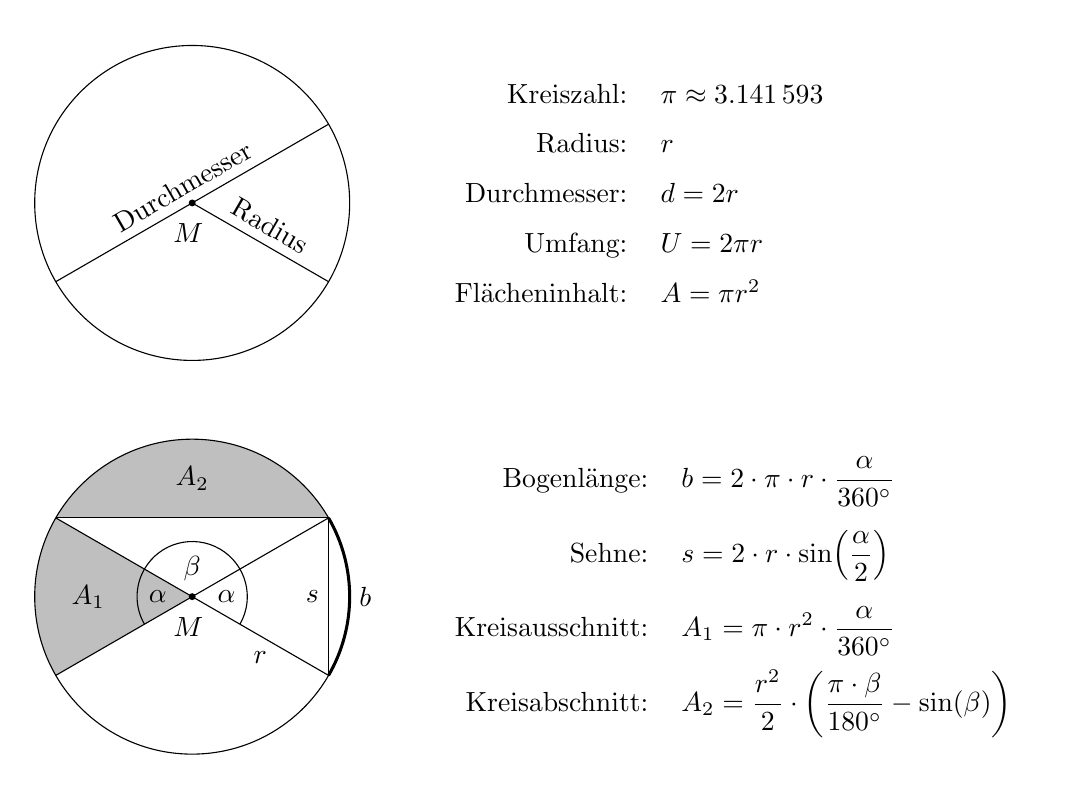
\begin{tikzpicture}
  \begin{scope}
    \fill (0, 0) circle[radius=1.25pt] node[below=4pt]{$M\;$};
    \draw (0, 0) circle[radius=2cm];
    \draw (0, 0) -- node[above, rotate=-30]{Radius} (330:2cm);
    \draw (210:2cm) -- node[above, rotate=30]{Durchmesser} (30:2cm);
    \node[right] at (3, 0)
    {%
      \begin{minipage}{22em}%
        \rule[-5.1\baselineskip]{0pt}{10\baselineskip}%
        \renewcommand{\arraystretch}{1.5}%
        \begin{tabular}{rl}%
          Kreiszahl:     & $\pi\approx\num{3.141593}$ \\
          Radius:        & $r$                        \\
          Durchmesser:   & $d=2r$                     \\
          Umfang:        & $U=2\pi r$                 \\
          Flächeninhalt: & $A=\pi r^2$
        \end{tabular}%
      \end{minipage}%
    };
  \end{scope}%
  \begin{scope}[yshift=-5cm]%
    \newcommand{\radius}{2cm};
    \coordinate (M) at (0, 0);
    \coordinate (A) at (-30:\radius);
    \coordinate (B) at (30:\radius);
    \coordinate (C) at (150:\radius);
    \coordinate (D) at (210:\radius);
    % Flaechen
    \fill[fill=black!25!white] (C) arc[start angle=150, end angle=210, radius=2] -- (M);
    \fill[fill=black!25!white] (B) arc[start angle=30, end angle=150, radius=2] -- cycle;
    \node at (-0.66*\radius, 0) {$A_1$};
    \node at (0, 0.75*\radius) {$A_2$};
    % Mittelpunkt
    \fill (M) circle[radius=1.25pt] node[below=4pt]{$M\;$};
    % Kreis
    \draw (M) circle[radius=2cm];
    % Kreisausschnitte
    \draw (A) -- node[below=2pt]{$r$} (M) -- (B);
    \draw (C) -- (M) -- (D);
    % Kreisbogen
    \draw[line width=1.1pt] (A) arc[start angle=-30, end angle=30, radius=2];
    \node[right] at (2, 0) {$b$};
    % Sehnen
    \draw (A) -- node[left]{$s$} (B);
    \draw (B) -- (C);
    % Winkel
    \draw (-30:7mm) arc[start angle=-30, end angle=210, radius=7mm];
    \node[right=2mm] at (M){$\alpha$};
    \node[above=2pt] at (M){$\beta$};
    \node[left=2mm] at (M){$\alpha$};
    % Formeln
    \node[right] at (3, 0)
    {%
      \begin{minipage}{22em}%
        \rule[-5.1\baselineskip]{0pt}{10\baselineskip}%
        \renewcommand{\arraystretch}{2.25}%
        \begin{tabular}{rl}%
          Bogenlänge:      & $\displaystyle b=2\cdot\pi\cdot r\cdot\frac{\alpha}{360^\circ}$ \\
          Sehne:           & $\displaystyle s=2\cdot r\cdot\sin\!\left(\frac{\alpha}{2}\right)$ \\
          Kreisausschnitt: & $\displaystyle A_1=\pi\cdot r^2\cdot\frac{\alpha}{360^\circ}$ \\
          Kreisabschnitt:  & $\displaystyle A_2=\frac{r^2}{2}\cdot\left(\frac{\pi\cdot\beta}{180^\circ}-\sin(\beta)\right)$
        \end{tabular}%
      \end{minipage}%
    };
  \end{scope}
\end{tikzpicture}

% ------------------------------
\section*{Äquivalenzumformungen}
% ------------------------------
\begin{center}
  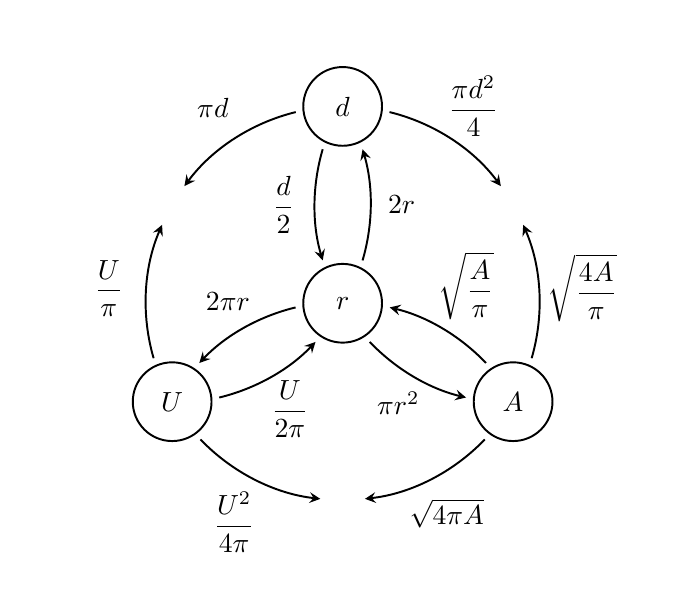
\begin{tikzpicture}[line width=0.7pt]
    \clip (-4, -3.5) rectangle (4, 3.5);
    \draw (0.00000, 0.00000) circle[radius=0.500cm] node{$r$};
    \draw (0.00000, 2.50000) circle[radius=0.500cm] node{$d$};
    \draw (-2.16506, -1.25000) circle[radius=0.500cm] node{$U$};
    \draw (2.16506, -1.25000) circle[radius=0.500cm] node{$A$};
    \draw[->, >=stealth] (-0.59566, 2.42800) arc[start angle=103.78421, end angle=143.48737, radius=2.50000];
    \draw[<-, >=stealth] (-2.29287, 0.99637) arc[start angle=156.51263, end angle=196.21579, radius=2.50000];
    \draw[->, >=stealth] (-1.80488, -1.72986) arc[start angle=223.78421, end angle=263.48737, radius=2.50000];
    \draw[<-, >=stealth] (0.28356, -2.48387) arc[start angle=276.51263, end angle=316.21579, radius=2.50000];
    \draw[->, >=stealth] (2.40054, -0.69814) arc[start angle=343.78421, end angle=383.48737, radius=2.50000];
    \draw[<-, >=stealth] (2.00931, 1.48750) arc[start angle=36.51263, end angle=76.21579, radius=2.50000];
    \node at (-1.64868, 2.47811) {$\pi d$};
    \node at (-2.97045, 0.18875) {$\displaystyle\frac{U}{\pi}$};
    \node at (-1.37727, -2.77886) {$\displaystyle\frac{U^2}{4\pi}$};
    \node at (1.32176, -2.66686) {$\sqrt{4\pi A}$};
    \node at (3.04530, 0.19350) {$\displaystyle\sqrt{\frac{4A}{\pi}}$};
    \node at (1.66253, 2.49892) {$\displaystyle\frac{\pi d^2}{4}$};
    \draw[->, >=stealth] (-0.25311, 1.95600) arc[start angle=163.59650, end angle=196.40350, radius=2.50000];
    \draw[->, >=stealth] (0.25311, 0.54400) arc[start angle=343.59650, end angle=376.40350, radius=2.50000];
    \draw[->, >=stealth] (-0.59767, -0.05280) arc[start angle=103.59650, end angle=136.40350, radius=2.50000];
    \draw[->, >=stealth] (-1.56739, -1.19720) arc[start angle=283.59650, end angle=316.40350, radius=2.50000];
    \draw[->, >=stealth] (0.34456, -0.49120) arc[start angle=223.59650, end angle=256.40350, radius=2.50000];
    \draw[->, >=stealth] (1.82050, -0.75880) arc[start angle=43.59650, end angle=76.40350, radius=2.50000];
    \node at (-0.75000, 1.25000) {$\displaystyle\frac{d}{2}$};
    \node at (0.75000, 1.25000) {$2r$};
    \node at (-1.45753, 0.02452) {$2\pi r$};
    \node at (-0.67003, -1.33947) {$\displaystyle\frac{U}{2\pi}$};
    \node at (0.70753, -1.27452) {$\pi r^2$};
    \node at (1.57003, 0.21937) {$\displaystyle\sqrt{\frac{A}{\pi}}$};
  \end{tikzpicture}
\end{center}

% ------------------------------------------------------------------------------
\end{document}
% ------------------------------------------------------------------------------

